
\documentclass{amsart}
\usepackage{amsmath}
\usepackage{amssymb}
\usepackage{amsthm}
\usepackage{hyperref}
\usepackage{tikz}\usetikzlibrary{positioning,decorations.fractals,decorations.pathmorphing}


\begin{document}
\title{Hello World}
\author{Peter Krautzberger}
\date{2025}

\maketitle

\section{Well hello there}

This is a simple test.


\begin{equation} \label{tikzPic}
    x = \begin{tikzpicture}[baseline=0pt]
        \draw (-1.5,0) -- (1.5,0);
        \draw (0,-1.5) -- (0,1.5);
    \end{tikzpicture}
\end{equation}
    

\begin{figure}
    \caption{An external graphic, Public domain \url{https://www.loc.gov/resource/mrg.06198/}{https://www.loc.gov/resource/mrg.06198/}}
    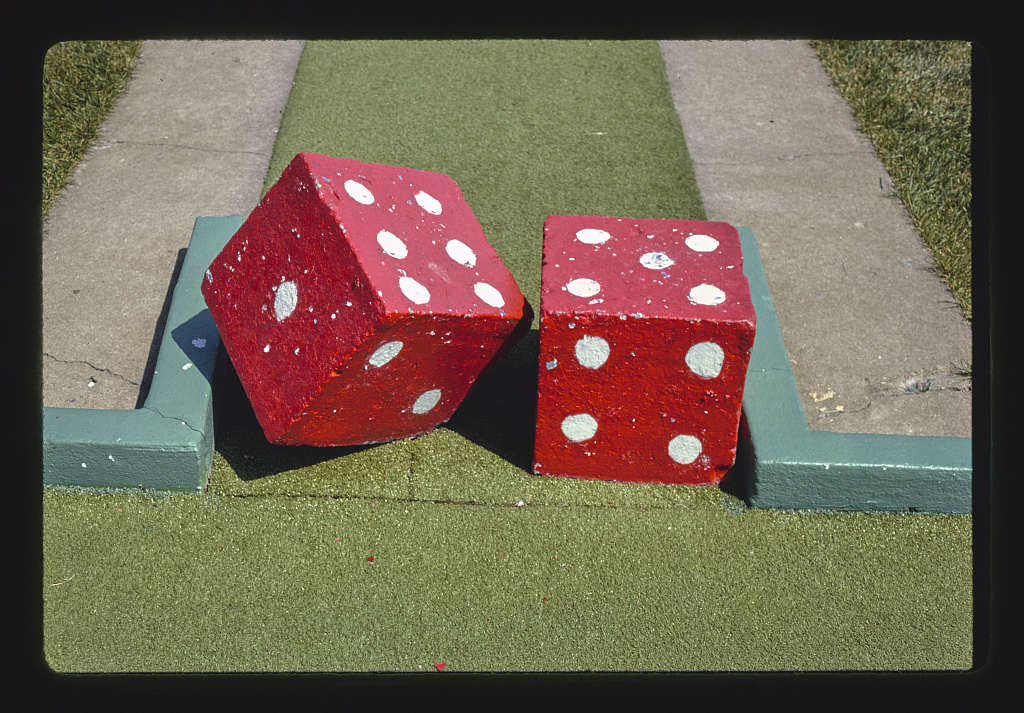
\includegraphics[width=.5\linewidth,alt={A photo of a minigolf obstacle consisting of a pair of large, red dice.}]{./Images/service-pnp-mrg-06100-06198v.jpg}
\end{figure}

\end{document}
